\chapter{MySQL Operator}

In this chapter the main part of the project is described. First we provide 
a high-level overview, followed by a detailed design of the \texttt{MySQL Operator} 
and \texttt{Backup Custom Resources}. Next, we present basic usage examples.

\section{High-level overview}
MySQL Operator allows a user to easily deploy replicated MySQL databases on a Kubernetes cluster.
It provides single-command cluster creation, scaling and backup scheduling. The project is divided
into two essential parts:
\begin{itemize}
	\item The actual operator --- a running service which listens for changes on Custom Resource
	objects and creates a new desired configuration on the Kubernetes cluster.
	\item A command line interface --- an optional tool facilitating interaction with the created
	resources.
\end{itemize}

In this chapter we will focus on the first one of mentioned elements.

\subsection{Functionalities}
The MySQL Operator allows the user to create, delete, update, backup and restore MySQL clusters.

When \textbf{creating} the cluster, the operator deploys a new instance of a replicated MySQL
database cluster alongside with all additional Kubernetes objects necessary for a proper deployment.
Additionally, rather than initializing a fresh cluster, data may be
\textbf{restored} from a backup file.

When a cluster is to be \textbf{removed}, the operator takes care to delete the cluster and its
configuration from Kubernetes. Unless explicitly specified, database data remains available, to be
cleaned up manually.

A running cluster may be \textbf{updated} by, for example, changing the configuration (port,
password) or scaling the cluster (increasing or decreasing the number of replicas deployed in the
cluster). When such an update is requested, the operator makes sure all the relevant Kubernetes
objects are updated to reflect the new cluster configuration.

We provided users with the ability to schedule backups. \textbf{Scheduling a backup} initiates a
recurring backup. The backup job’s behavior is similar to a cron job’s -- backups are created
cyclically at regular intervals.

\section{Project Design}

\subsection{Custom Resource Definition design}
The main custom resource provided by our project is \texttt{MySQLCluster}. A Custom Resource of this kind
represents a cluster of replicated MySQL servers. It has a unique name specified by the user and
that name also becomes the name of a Kubernetes Service through which the database is exposed.
Another Custom Resource defined in our project is \texttt{MySQLBackup}. Objects of this kind are created when
the user wants to schedule database backups. Each instance of this resource corresponds to a backup
schedule request for a specific cluster.

\subsection{Design Patterns}
The MySQL Operator’s implementation is primarily based on two common Kubernetes design patterns:
the controller and operator patterns. A \textbf{controller} is an informer whose responsibility is
to monitor changes in an application’s state. On each change, a predefined controller function is
executed. An \textbf{operator} builds on ideas from the controller pattern and basic Kubernetes
concepts. It is responsible for creating, configuring and managing stateful applications running on
clusters. Operators extend the Kubernetes API and create multiple instances of applications like
core Kubernetes resources.

\begin{figure}[!ht]
    \centering
    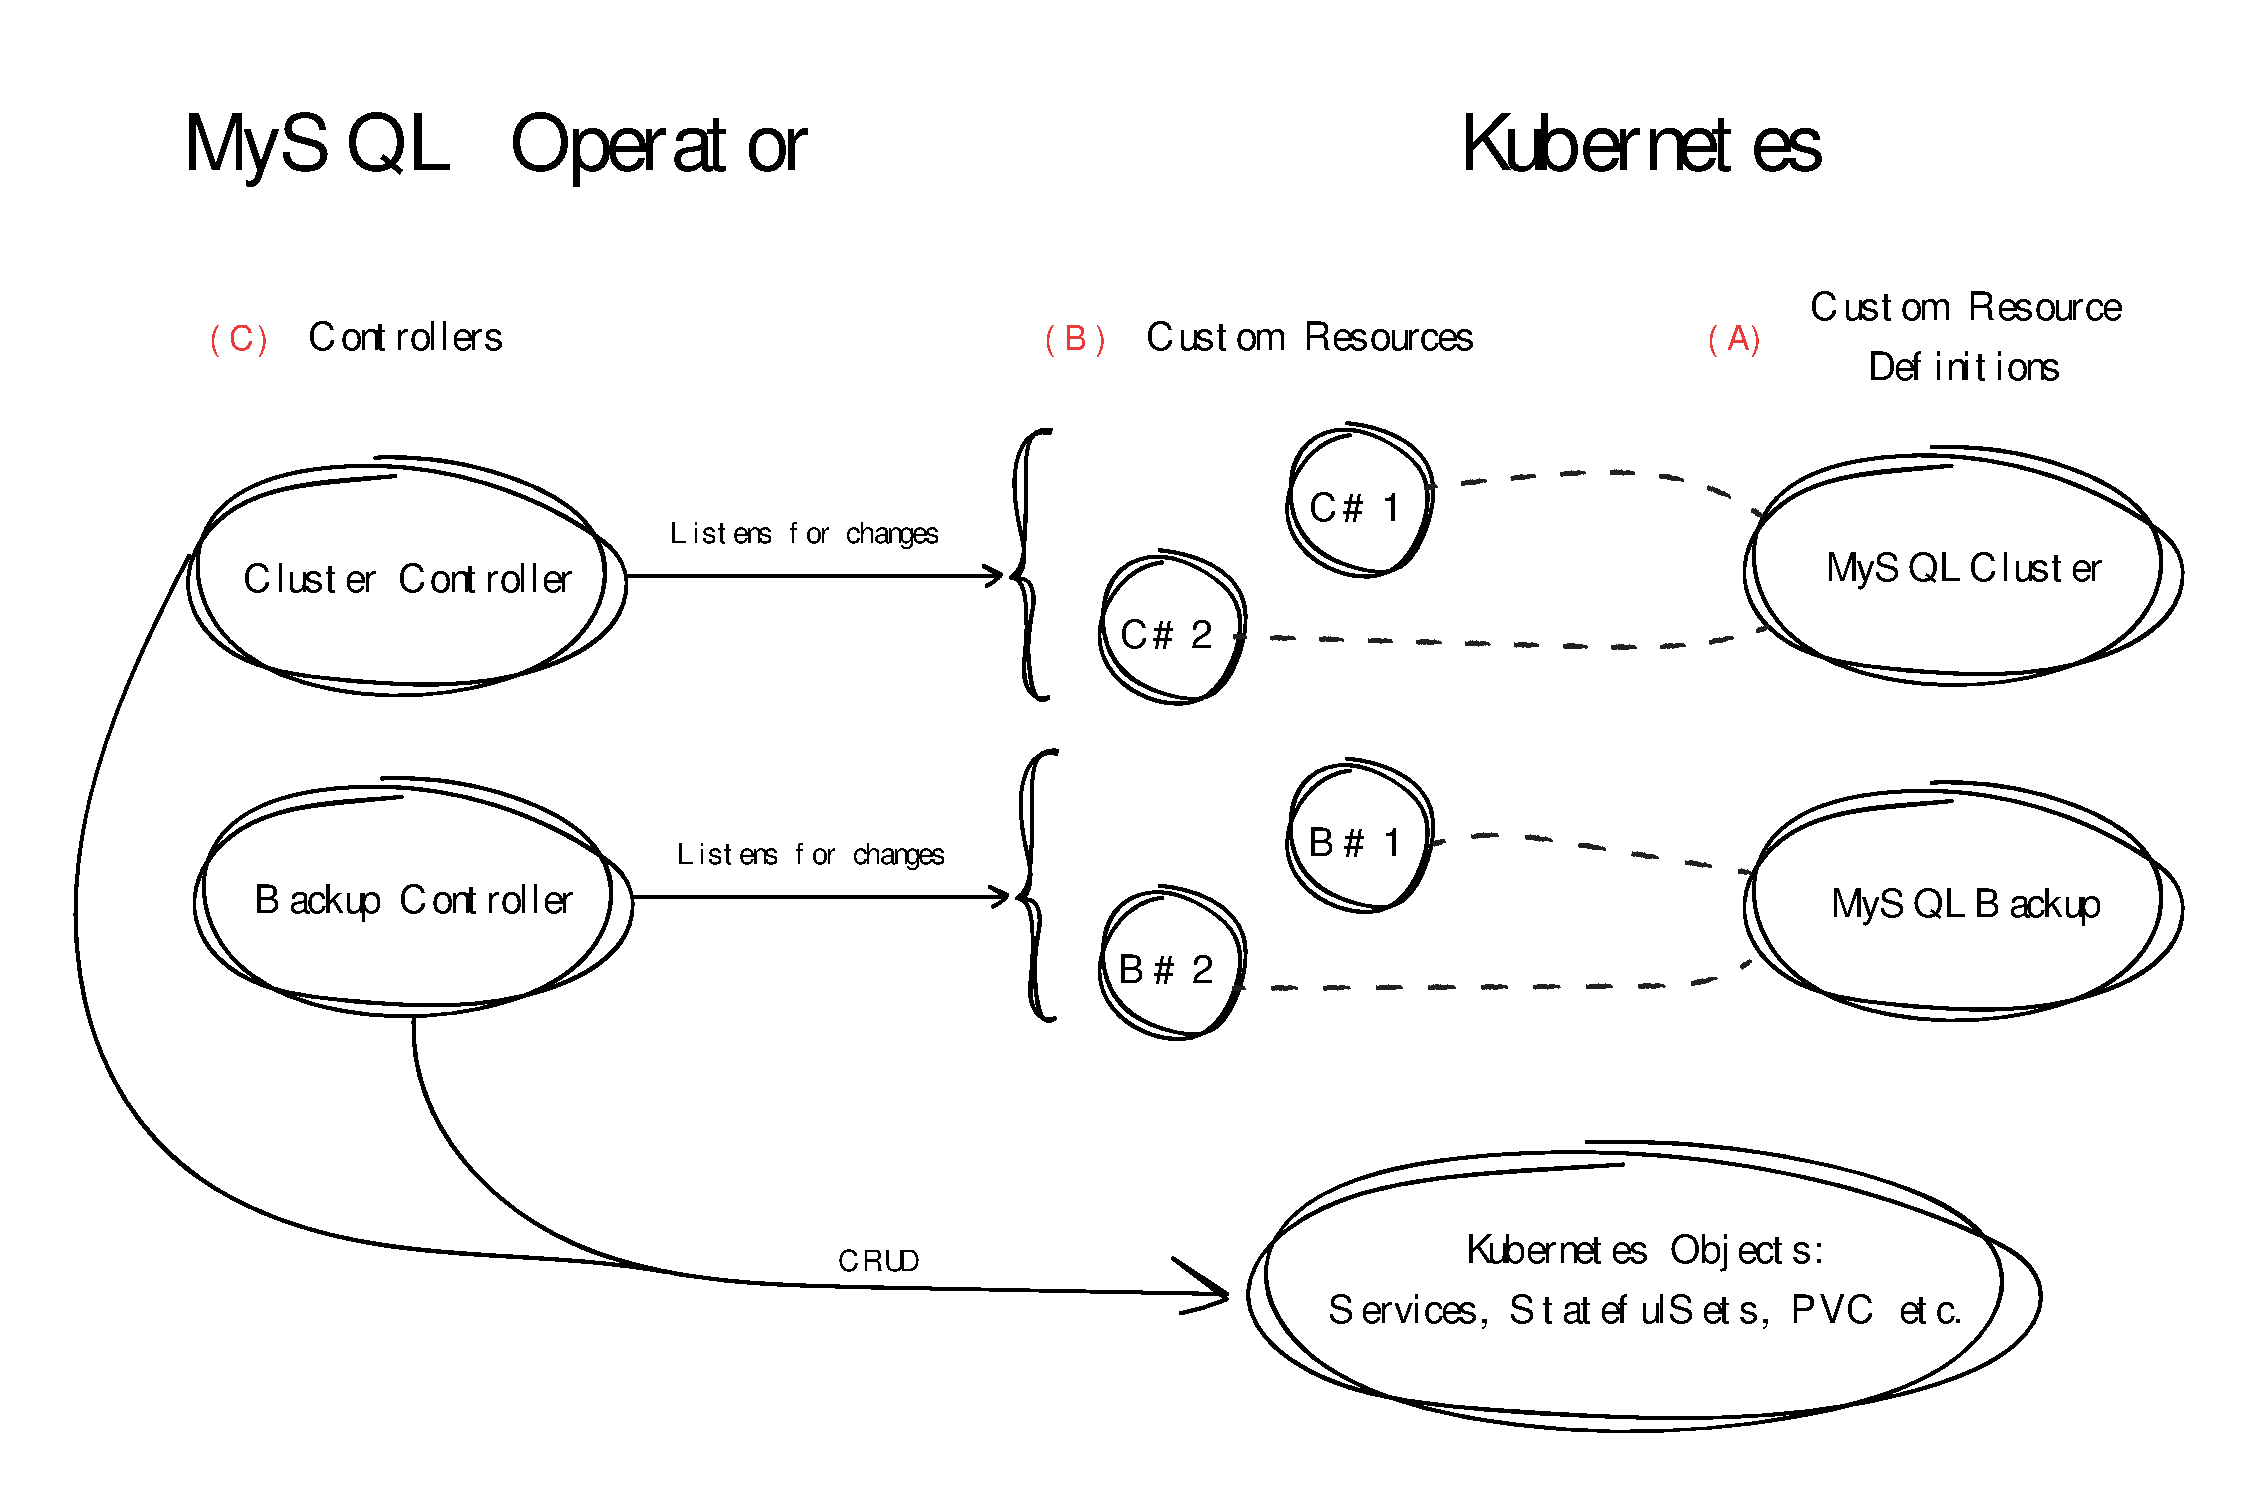
\includegraphics[width=1\textwidth, angle=0]{img/Design.pdf}
    \caption{MySQL operator architecture}
    \label{fig:design}
\end{figure}

To get a better understanding of the controller and operator design patterns, let’s look at an
example of how an operator will respond to a user’s action. Let’s say the user wants to modify a
\texttt{MySQLCluster} instance. From the user’s point of view, this can be done by issuing a
\texttt{kubectl patch} command. From the operator’s point of view, an \textit{Update} event is
received and the corresponding operator handler is called by the controller.

We use the controller and operator patterns to manage resources related to both 
\texttt{MySQL servers} and \texttt{backup jobs}. A high level overview of the project design is
illustrated in Figure \ref{fig:design}. During operator startup, two
\texttt{CustomResourceDefinitions} (figure \ref{fig:design} A) are registered into the Kubernetes API.
From this point on, users can define their own Custom Resource instances (Figure \ref{fig:design} B) ---
\texttt{MySQLClusters} (ex. C1, C2) and \texttt{MySQLBackupSchedules} (ex. B1, B2). Each kind of
Custom Resource has its corresponding controller listening and reacting to changes on these
resources. The cluster controller and the backup controller (Figure \ref{fig:design} C), though technically
goroutines\footnote{Function or methods that run parallel with other functions or methods.} in a single
MySQL Operator process, can be thought of as separate processes responsible for separate parts of the
cluster’s architecture. Thanks to these constructs we can monitor custom resource instances and adjust
all the related objects as necessary. The operator pattern was designed for stateful applications, making
it suitable for both database cluster and backup management.~\cite{coreos}

\subsection{Detailed design of the MySQL cluster}

\subsubsection*{Create}
The internal implementation of a \texttt{MySQLCluster} within Kubernetes consists of two parts. First,
several Pods (one for each replica) running a containerized MySQL server are managed by a
StatefulSet. Secondly, two Kubernetes Services expose the MySQL servers as named endpoints by
configuring Kubernetes’ DNS. Two distinct Services are necessary because different nodes in the
cluster have different capabilities. Specifically, the master node is the only one to which writing
is allowed. Therefore, one Service exposes only the  master node and allows for both reading and
writing, while the second Service connects to all nodes, but allows for read-only access. 

Our operator is responsible for creating the appropriate StatefulSet and Services when the user
creates a \texttt{MySQLCluster} object.

\subsubsection*{Services}
A Service object represents the network configuration necessary to expose a specific service at a
particular domain name and port. To expose the \texttt{MySQLCluster} we create what’s called a
“headless Service.” No specific IP address is configured. Instead, we specify which Pods (the ones
managed by our StatefulSet) should be available under the given address. The Service then configures
Kubernetes’s DNS to return an \textbf{A record}\footnote{An \textbf{A record} maps a domain name to
the IP address (IPv4) of the computer hosting the domain.} pointing at each of the Pods. This
essentially means that DNS load balancing is used to load balance queries to the database cluster.

\subsubsection*{Delete}
When a \texttt{MySQLCluster} instance is deleted, all the related objects should be cleared from Kubernetes
as well. Thanks to the \texttt{ownerReferences} attribute, we do not have to worry about manual
deletion of dependent structures. Kubernetes understands that some objects are owned by others, and
when a parent object is deleted, the children will be deleted as well. Thus all we have to do is to set
the \texttt{ownerReferences} field of the Services and StatefulSet we create to the parent
\texttt{MySQLCluster} object’s UID and Kubernetes will take care of garbage collection for us.

Objects which are meant to have a longer lifetime, such as \textit{PersistentVolumeClaims} and the
\textit{PersistentVolumes} on which database data is stored, will not be deleted. In order to
proceed with a hard delete, these constructs have to be removed separately.

\subsubsection*{Scale/Update}
The operator’s update handler receives information about how the cluster’s configuration looked
like before the update, and what the new requested configuration is. Based on this, we can create
new configurations for the cluster’s related objects (the Services and StatefulSet) and issue update
requests for those. In case of an error, we update the \texttt{MySQLCluster’s} status field with an error
message. The cluster might be partially updated and its previous state is not reinstated.

\begin{figure}[!ht]
    \centering
    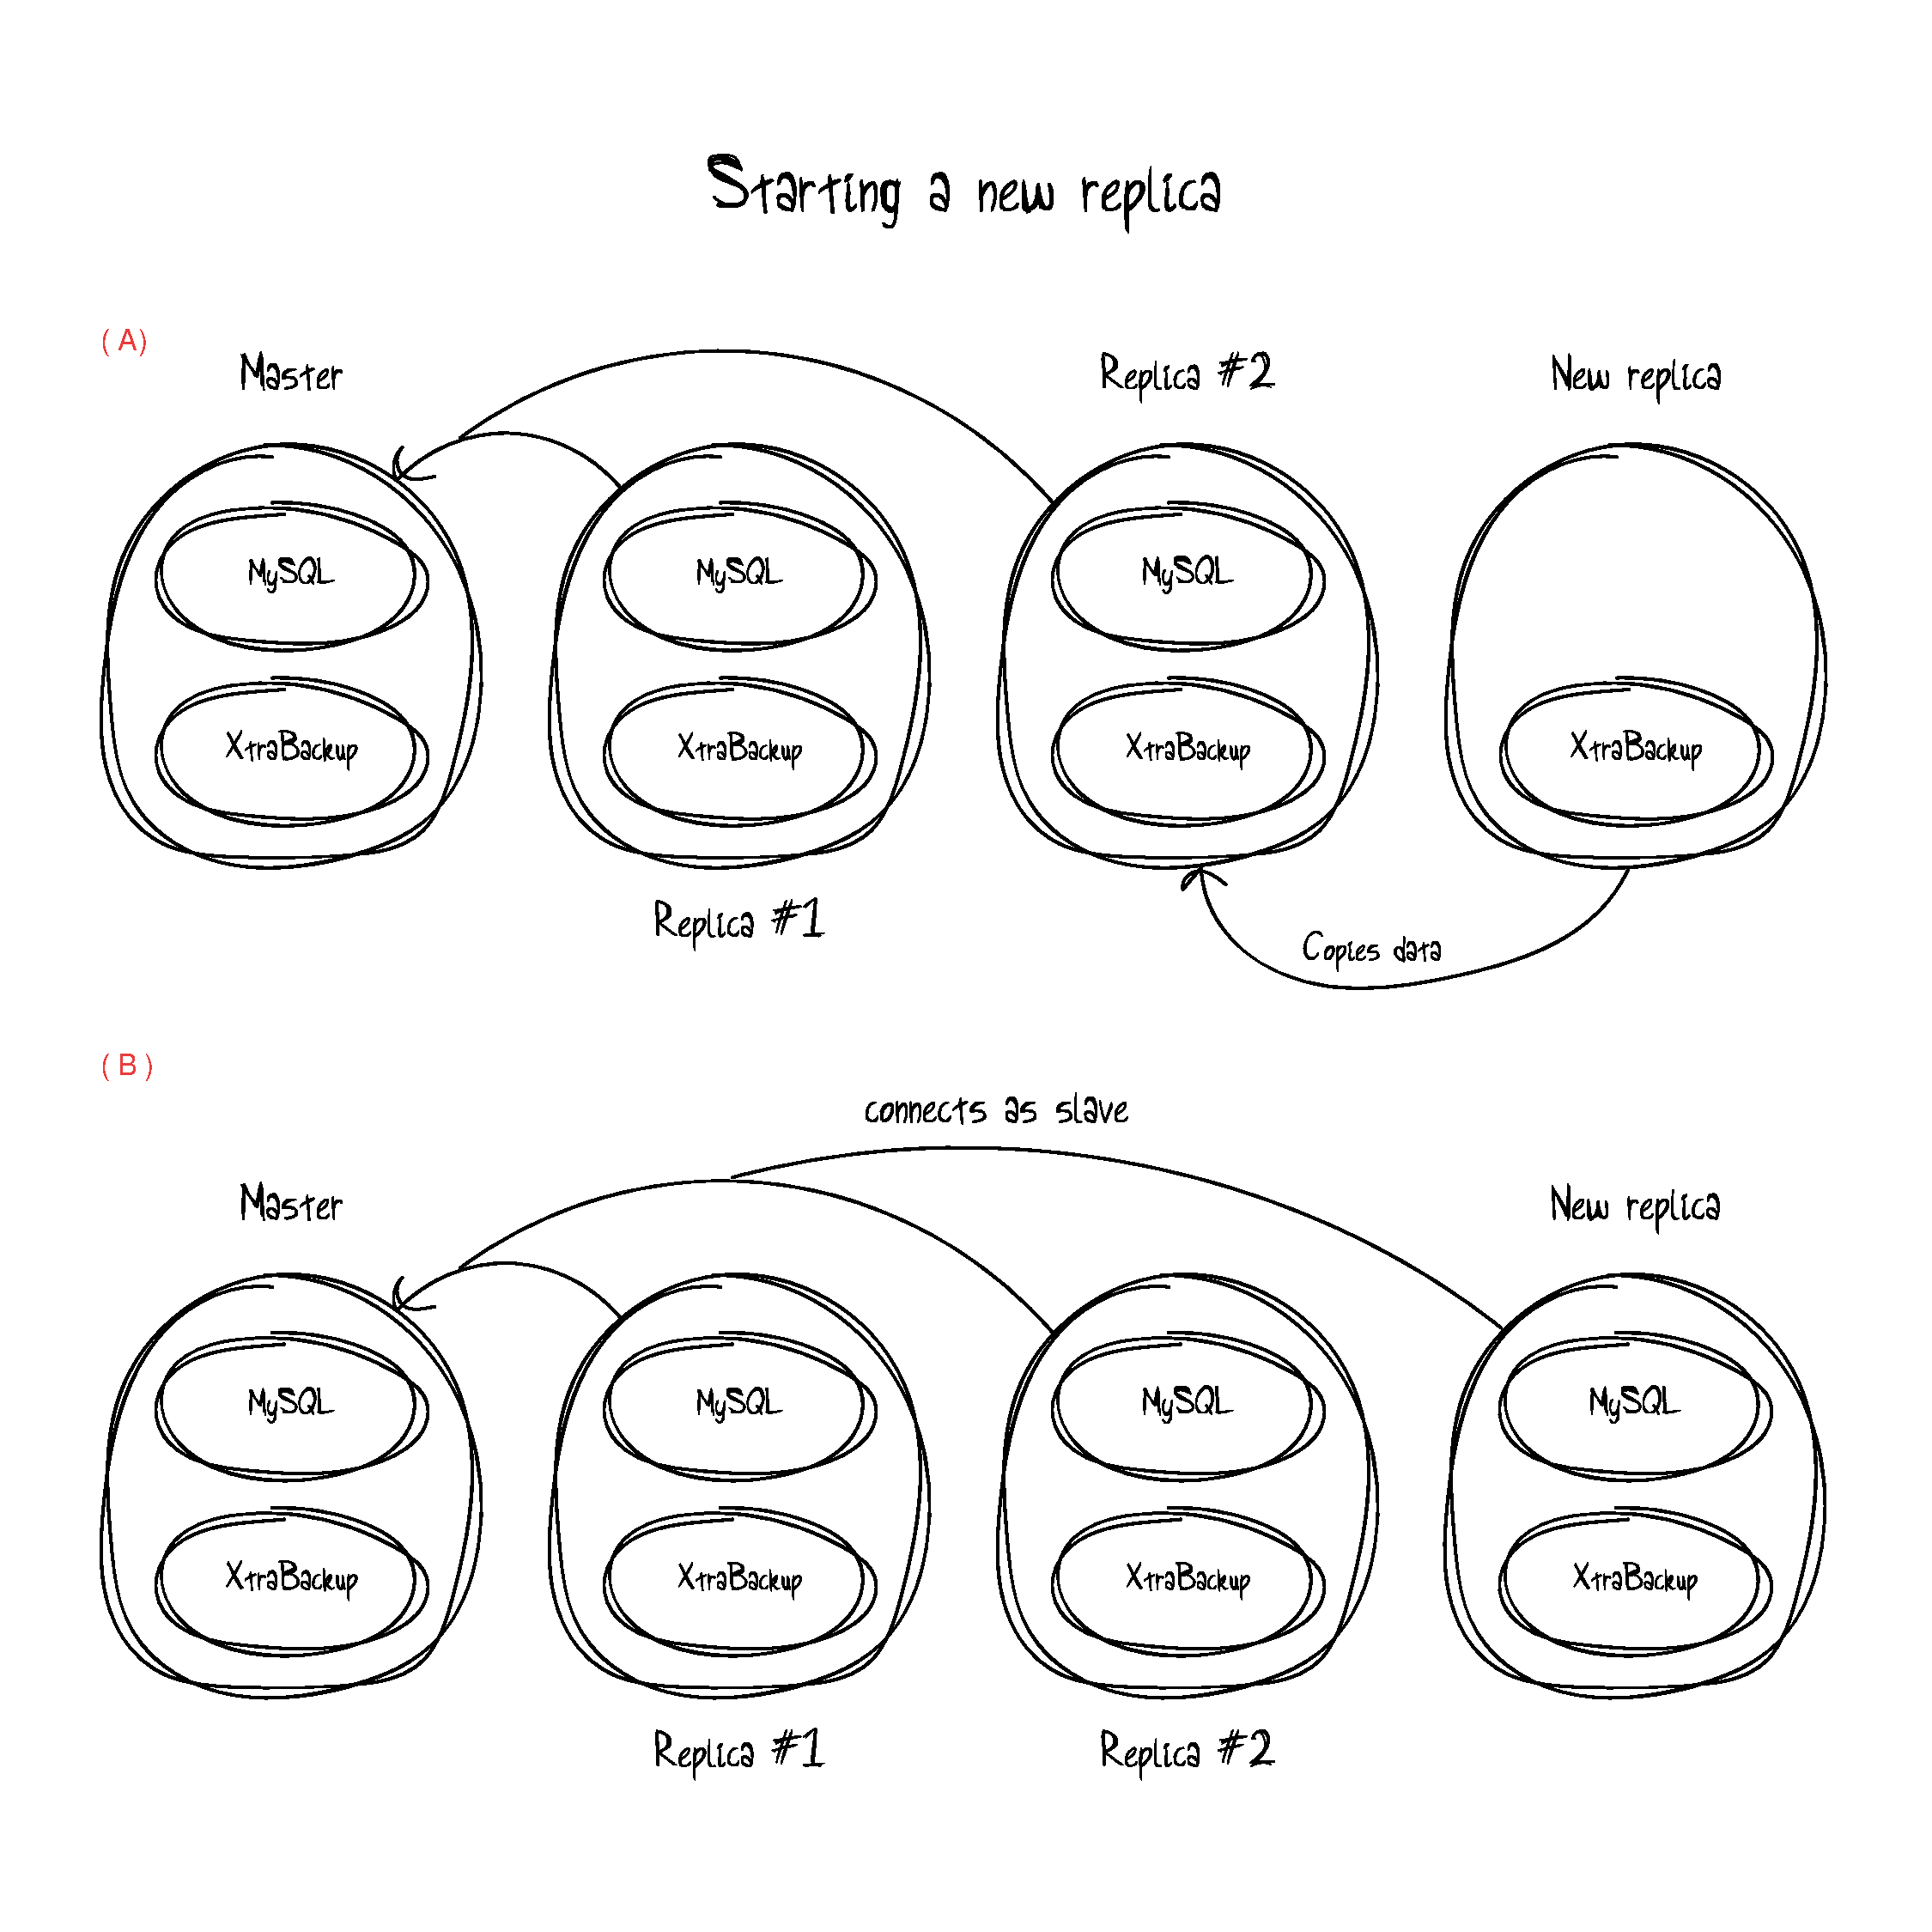
\includegraphics[width=1\textwidth, angle=0]{img/replication.pdf}
    \caption{Replication}
    \label{fig:replication}
\end{figure}

Core Kubernetes structures, such as StatefulSets or Services, are already equipped with mechanisms
for scaling and configuration updates that do most of the work for us (for example, starting up new
Pods if the replica count is increased). However, when scaling up, we need to copy the cluster’s
data to the newly created replicas. To achieve non-blocking replication, every pod has an XtraBackup
container running beside the main MySQL server container. \textbf{Percona XtraBackup}~\cite{percona}
is a popular, lightweight, and easy to use program that replicates data from a database without
stopping it. When a new Pod in a StatefulSet is created, its initial data is copied from the
previous Pod by connecting to its XtraBackup (exposed via \textbf{ncat}\footnote{Tool to read from and
write to network connections using UDP or TCP.}) --- each new replica copies the data from its direct
predecessor (Figure \ref{fig:replication} A). This allows us to avoid overloading the master node,
which would have occurred if the replica nodes all copied data from it. A new replica is then connected
as a slave to the master MySQL server (Figure \ref{fig:replication} B).

\section{Detailed design of the MySQL backups}

\begin{figure}[!ht]
    \centering
    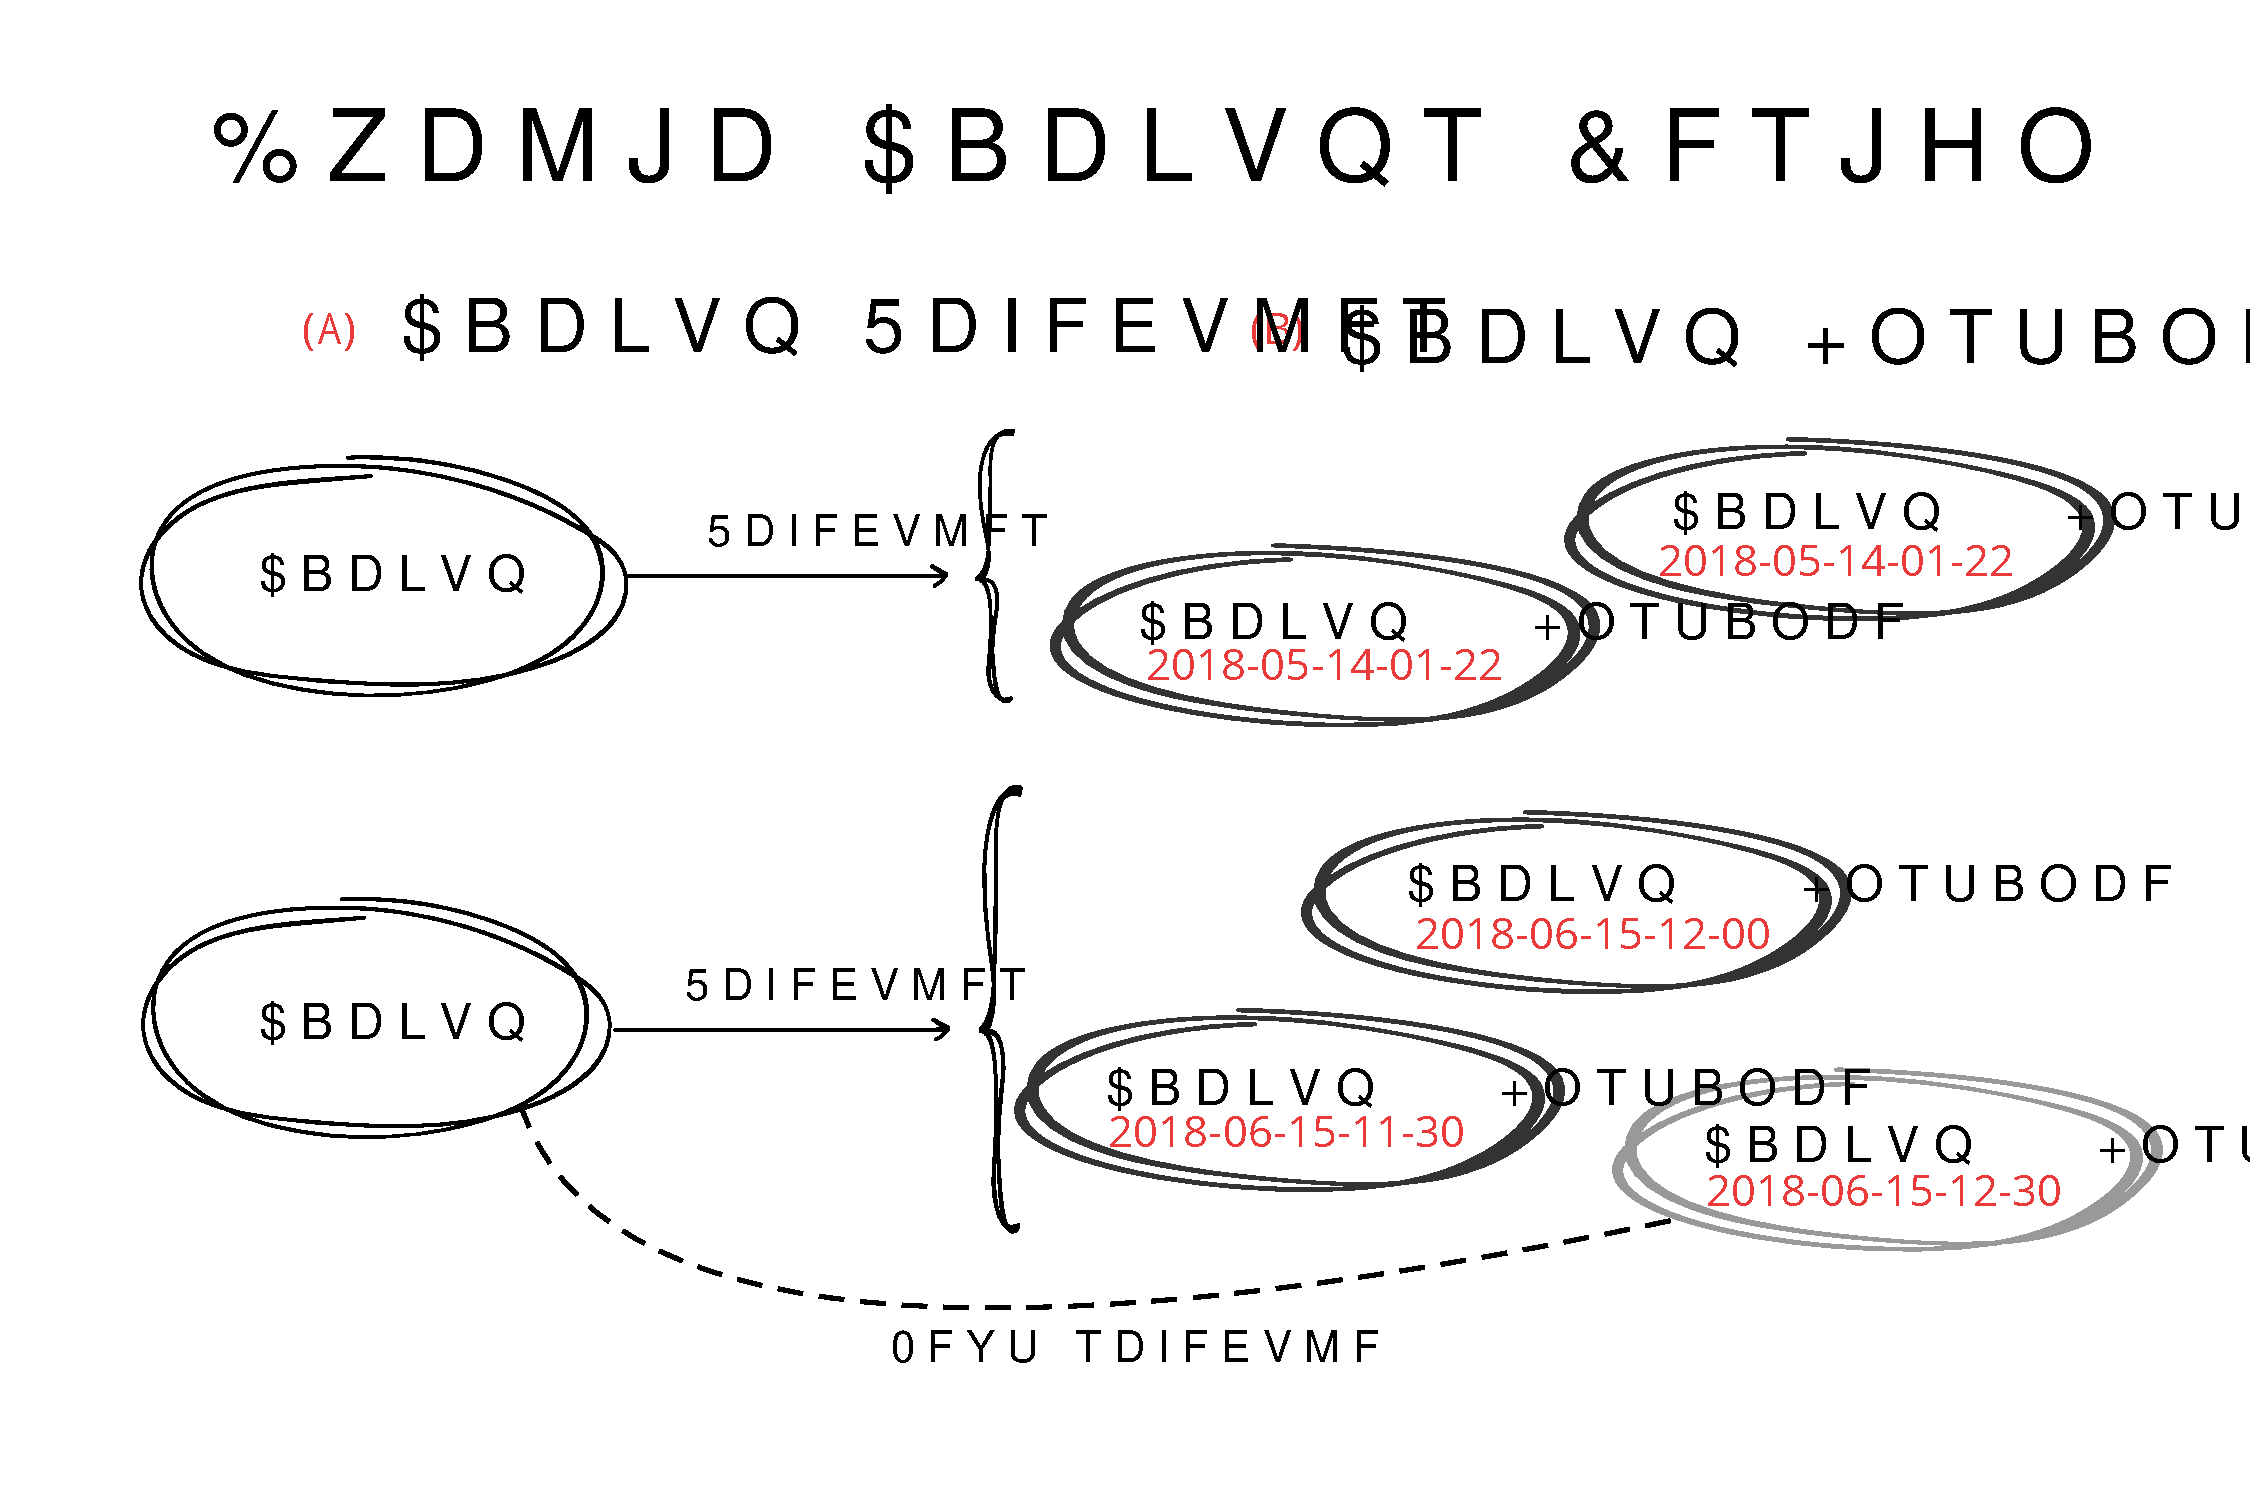
\includegraphics[width=1\textwidth, angle=0]{img/cyclic_backups.pdf}
    \caption{MySQL backup design}
    \label{fig:backups}
\end{figure}

\subsubsection*{Backup}
In order to provide users with cyclic backups of a MySQL cluster, we created 
two separate CustomResourceDefinitions: \texttt{MySQLBackupSchedule} and 
\texttt{MySQLBackupInstance}. Objects of the first type are responsible for 
scheduling and managing the groups of backups. At the same time, objects 
of the latter type reflect the actual backups created. As a result, each 
of the \texttt{MySQLBackupSchedules} can have multiple corresponding 
\texttt{MySQLBackupInstances} --- one for each backup created.

To gain a better understanding of this structure, let’s analyse the Figure 
\ref{fig:backups}. From the user point of view, cyclic backups are requested 
by creating a \texttt{MySQLBackupSchedule} object (A). Backup creation is handled 
by a Kubernetes CronJob object created by our operator. A CronJob periodically 
creates Kubernetes jobs which run to completion. In our case, each of these 
jobs creates a separate MySQLBackupInstance object (B). After that, the 
dedicated operator creates an actual backup without overwriting previous 
backups. The status of a \texttt{MySQLBackupInstance} object reflects the state of 
an actual backup --- the user can see if certain backup succeed. Thanks 
to this design it is also fairly easy to list all the existing backups, 
it’s simply listing the \texttt{MySQLBackupInstance} objects.

All the backups for a single MySQLBackupSchedule are stored in a single 
PersistentVolume. The backed up data is not deleted when the cron job is 
cancelled since PersistentVolumes are not owned by our object.

For the actual backup creation we reuse the solution applied for scaling 
up MySQL clusters. The backup mechanism utilizes the same XtraBackup endpoints 
to get the data from our database. Backups are always based on the master 
node’s data.


\subsubsection*{Restore}
Users can restore any backup instance from a chosen backup schedule. This is simply done by creating
a new \texttt{MySQLCluster} object with the name of the backup to restore from specified in the
configuration.

\section{Use Cases}
In order for the custom resources to be properly processed and an actual MySQL cluster deployed, a
running instance of the MySQL Operator is required inside the Kubernetes infrastructure. The
recommended option is to start a MySQL Operator image as a Deployment in the cluster:

\texttt{kubectl run mysql-operator --image=grtl/mysql-operator:latest}

\subsection{Cluster}
\subsubsection*{Create/Restore}

The \texttt{MySQLCluster} creation is the most essential part of the 
workflow. At this point user has to decide on cluster configuration.

\begin{lstlisting}
> kubectl create secret generic my-password \
	--from-literal=password="password"

> kubectl apply -f cluster-config.yaml
\end{lstlisting}

\paragraph{Data to specify}
\begin{enumerate}
	\item Cluster name.\footnote{Cluster name must be unique, it will be the future reference
	to the cluster.}
	\item Root password \textit{(Kubernetes secret)}.
	\item MySQL port \textit{(optional, defaults to 3306)}.
	\item Number of replicas \textit{(optional, default to 2)}.
	\item Storage size \textit{(optional, default to 1Gi)}.
	\item Custom \textbf{mysql} image. \textit{(optional)}.
	\item Backup name \textit{(optional)}.\footnote{If provided, initial cluster data is restored
	from backup}
\end{enumerate}

\paragraph{Example \textbf{cluster-config.yaml}}
\begin{lstlisting}[caption=cluster-config.yaml,captionpos=b]
apiVersion: cr.mysqloperator.grtl.github.com/v1
kind: MySQLCluster
metadata:
  name: "my-cluster"
spec:
  name: "my-cluster"
  password: "my-password"
  port: 3306
  storage: 1Gi
  mysqlImage: "mysql:latest"
  restoreFrom: 
	backupName: "my-backup"
	instance: "2017-12-14-01-22"
\end{lstlisting}

\subsubsection*{Delete}

It is possible to delete many clusters at the same time by simply writing
names of all the clusters we want to remove from Kubernetes.

\begin{lstlisting}
> kubectl delete mysqlcluster my-cluster
OR
> kubectl delete mc my-cluster
\end{lstlisting}

\paragraph{Data to specify}
\begin{enumerate}
	\item Cluster name \textit{(one or more)}.
	\item Persistent Volume Claims \textit{(optional)}.
\end{enumerate}

\subsubsection*{Update}

Not every element of configuration can be updated. Even though we aimed 
to provide the best configurability possible, users cannot modify the
cluster name.

\begin{lstlisting}
> kubectl apply -f cluster-config.yaml
\end{lstlisting}

\paragraph{Data to specify}
\begin{enumerate}
	\item Cluster name.
	\item Root password \textit{(Kubernetes secret, optional)}.
	\item MySQL port \textit{(optional)}.
	\item Number of replicas \textit{(optional)}.
\end{enumerate}

\subsection{Backup}
\subsubsection*{Create}

During the backup creation users specify how often they want their backups 
to be created.

\begin{lstlisting}
> kubectl create -f backup-config.yaml
\end{lstlisting}

\paragraph{Data to specify}
\begin{enumerate}
	\item Backup name \textit{(optional: defaults to auto generated based on cluster name)}.
	\item Cluster name.
	\item Time \textit{(CRON style, required)}.
	\item Storage \textit{(optional: default to the Cluster storage size)}.
\end{enumerate}

\noindent  \textbf{Additional info}

\noindent Database will be backed up in an automatically claimed Persistent Volume with the size
calculated based on the cluster current database size.

\paragraph{Example \textbf{backup-config.yaml}}
\begin{lstlisting}[caption=backup-config.yaml,captionpos=b]
apiVersion: cr.mysqlbackup.grtl.github.com/v1
kind: MySQLBackupSchedule
metadata:
  name: "my-backup"
spec:
  cluster: "my-cluster"
  time: "59 23 31 DEC Fri *"
  storage: 1Gi
\end{lstlisting}

\noindent  \textbf{Getting backup instances}

\noindent For getting created backup instances with a valuable output we recommend
using output flag with the following configuration:

\begin{lstlisting}
kubectl get mbi -o custom-columns="NAME:metadata.name,\
	STATUS:status.phase,SCHEDULE:spec.schedule,\
	CLUSTER:spec.cluster,CREATED:metadata.creationTimestamp"
\end{lstlisting}

\noindent Sample output:
\begin{lstlisting}
NAME          STATUS    SCHEDULE  CLUSTER    CREATED
bckp-instance Completed bckp      my-cluster 2018-04-27T14:42:33Z
\end{lstlisting}

\subsubsection*{Delete}

Deletion of the backups works in the same way as the cluster deletion.

\begin{lstlisting}
> kubectl delete mysqlbackupschedule my-backup
OR
> kubectl delete mbs my-backup
\end{lstlisting}

\paragraph{Data to specify}
\begin{enumerate}
	\item Cluster name \textit{(one or more)}.
	\item Persistent Volume Claims \textit{(optional)}.
\end{enumerate}

\subsubsection*{Update}

For backups the only value users can update is the backup 
scheduling time.

\begin{lstlisting}
> kubectl apply -f backup-config.yaml
\end{lstlisting}

\paragraph{Data to specify}
\begin{enumerate}
	\item Time \textit{CRON style}.
\end{enumerate}
